\chapter{Selection Application}
\label{sec:selection_application}

In this chapter, I will describe the implemented selection application used for this work. After a rundown of third party requirements and a summery of relevant C++ classes the description will be further segmented subdivided according to its abstract, key requirements.
The goal of this chapter is to describe how the application, especially the Octree\cite{Octree} was designed and implemented. Accordingly, key lines of source code as well als plenty of explanatory comments will be provided.

\section{Additional Third Party Libraries}
\label{sec:additional_third_party_libraries}

To ensure a scalable, platform independent implementation of the application, the following third party libraries, frameworks and APIs were used.

\subsection{OpenGL}
\label{sec:opengl}

The Open Graphics Library OpenGL \cite{OpenGL} is a powerful, industry standard API for rendering 2D and 3D grahpics, independently of programming language and operating system. One of its most outstanding features is its ability to directly perform operations on the graphics processing unit of a pc, allowing fast, hardware-accelerated display of graphic elements. For this work, openGL was used for displaying the 3D objects both in the user study and throughout development of the selection application. The task of displaying rendered images across multiple projection surfaces on a 360\degree panorama view was handled by software developed at the Zentrum f\"ur Virtuelle Realit\"at und Visualisierung (V2C) of the Leibniz-Rechenzentrum \cite{v2c}.

OpenGL is based on the following basic structures and concepts.

\begin{description}
	\item[Vertex Array Objects] (VAOs) are objects which can contain one or more Vertex Buffer Objects and store information for complete, rendered objects. In other words, VAOs store descriptions of vertex data stored in VBOs. For example, the number of coordinates the vertices are made of, in which order etc. From a performance aware point of view, they are a great improvement over older, deprectecated concepts in OpenGL since multiple calls to bind and upload distinct sets of data belonging to the same object to the graphics processing unit can be bundled in one call to a VAO.
	\item[Vertex Buffer Objects] (VBOs) contain the actual vertex data. Coordinates, normal and color information, texture mapping and any other kind of data that is desired can be saved in these kinds of objects. They are designed as buffer objects to be stored directly within the memopry of the video card, ensuring extremely fast access times.
	\item[Vertex Shaders] are small pieces of C-like code which can perform fast, basic operations on every vertex of a vertex data input stream. They are fed vertex attribute data, as specified in a VAO by the call of a openGL draw function. In many cases, vertex shaders will solely compute the position of 3D data on a 2D screen as well as paint it in basic colors. For more complex applications, vertex shaders can also perform super fast manipulation of large amounts of vertex data to achieve transitions in geometry, texture mapping, directions of normals \dots
	\item[Fragment Shaders] Fragments, not to be confused with triangles or faces, are sets of values resulting from rasterisation. They are frequently, informally described as \textit{potential pixels}, meaning the color value they describe, is what could be seen on a screen at a specific pixel under certain circumstances. For each fragment, one or more sets of values may be computed and things like lighting and postprocessing effects, bump maps, antialiasing or simply occlusion by another object may be determining factors as to which one will be rendered to one specific pixel on the output screen. Fragment shaders are used to define how color values for fragments will be selected to be displayed at their respective pixel.
\end{description}

\subsection{GLUT}
\label{sec:glut}

As stated on its official webpage \cite{GLUT}, GLUT is an official OpenGL Utility Toolkit which provides, among other features, support for multiple windows, control of such windows and handling input from devices such as keyboards and mouses. It is commonly used to achieve interactive windows with cross-platform compatibility displaying rendered images produced by OpenGL. Handling input via the handheld controller in the user study was achieved with the help of GLUT during this work.

\subsection{GLEW}
\label{sec:glew}

The OpenGL Extension Wrangler Library (GLEW)\cite{GLEW} is a cross-platform extension loading library, specifically designed to be used by C/C++ applications. It provides run-time mechanisms for OpenGL extensions supported on the target platform, allowing to faster query and load those extensions.

\subsection{ASSIMP}
\label{sec:assimp}

Available across multiple operating systems including Android and iOS, The Open Asset Import Library \cite{ASP}, is a powerful open source library that offers import, export and post-processing functions for most commonly used 3D data formats. In this work, its easy to use import function for OBJ files was used loading the 3D objects to be displayed in the user study. ASSIMP implements a set of hierarchically organised data structures or so-called nodes. Two of the most relevant ones for this work will be briefly described below.

\begin{description}
	\item[aiScene] is the root of all the imported data returned from a successful call to one of ASSIMPs import functions. Global information such as the direction of the coordinate system, its origin location as well as references to all the other data in the scene are stored here.
	\item[aiMeshes] represent imported meshes within the scene. Each aiMesh has its own local coordinate system with an origin point and all the vertices belonging to it. Multiple sets of data describing one imported mesh can be stored in these mesh objects but sets of vertices and faces are always guaranteed to be present, thus enabling a basic graphic representation of the mesh.
\end{description}

\section{Relevant Class Files}
\label{sec:relevant_class_files}

This section will cover all the relevant C++ classes used to implement the selection application. Note that these descriptions will only cover the general structure and purpose of these classes within the context of the applicatoin. For a more detailed description of the most crucial functions as well as a complete UML diagram representation of the application, please refer to \hyperref[sec:key_features]{Key Features}.
% @TODO "UML diagram" *hust*

\subsection{Object}
\label{sec:object}

The object class is used to represent a 3D object within the project. It uses import functions from ASSIMP to load a file via a given source path. An object can contain multiple mesh objects, segmentation happens automatically based on a threshold number of vertices that can be stored in one mesh. This class is used to work with potentially very large 3D files in a uniform and quick way, mostly by implementing wrapper functions that have each mesh object associated to an object call their upload and draw functions, their destructors etc.

\subsection{Mesh}
\label{sec:mesh}

One object can consist of multiple meshes. These meshes are coherent with instances of aiMesh (see \hyperref[sec:assimp]{ASSIMP}) and all the important attributes such as vertices, faces, normals, texture coordinates and IDs are stored here. OpenGL functions such as uploading vertex buffer data to the graphics proccessing unit and drawing are implemented here. Some of the applications most crucial functionalities such as adding to and removing vertices from the global selection of vertics to be highlighted are implemented in this class, see \hyperref[sec:key_features]{Key Features}.

\subsection{ocTree}
\label{sec:octree}
Spatial indexing of loaded objects in the application is entirely handled in this class. It has been one of the most labour-intensive parts of the application since formal guides to implementing it, independent of coding language, are next to non-existent and working with the data that was stored in the object and mesh classes above required an extensive amount of customisation.
% aktuell noch ocTreeLeaf

\section{Key Features}
\label{sec:key_features}
This section will describe the following features and functionalities which are most crucial to the selection application.

\begin{itemize}  
	\item Spatial indexing via ocTree
	\item User selection
	\item Tracking selection
	\item Testing setup 
\end{itemize}

\subsection{Spatial Indexing via Octree}
\label{sec:spatial_indexing_via_octree}

As mentioned above, the \texttt{ocTree} class handles spatial indexing and, therefor, provides quick access to every vertex of an imported 3D object via a set of integer-like (\texttt{size\_t}) indices. The general approach to this implementation of the concept of ocTrees was desigend with a heavy emphasis on its recursive features. Instances of it can be created from everywhere in the application by the call of its public root constructor function. Nodes can be leafs or not, which is indicated by a boolean flag for every instance of an \texttt{ocTree} object. Leaf nodes do not have subtree-nodes that refer to them as parents, they solely save vertices within their bounds. Non-leaf nodes have eight children nodes, in other words, eight more \texttt{ocTree} objects which refer to them as their parent node.

For better understanding during development and clearer, human-readable log messages, the unique, binary identifiers were implemented with care. Each node of the tree has a private \texttt{std::vector} which serves as a unique combination of boolean values describing its identifier. It can be used for directly accessig any desired \texttt{ocTree} (subtree) object within a tree through its root node.

Starting from the root node (level \textit{l} = 0), such an identifier \textit{Id} with a length of \textit{n} boolean values can be used for locating the respective node within 3D space by considering three of its consecutive values at any time. At any level \textit{l}, those  values of \textit{Id} can be found at positions \textit{l*3}, \textit{l*3+1} and \textit{l*3+2} within it. If \textit{l*3+2} equals its length \textit{n}, the search ends and the resulting node can be queried for the vertices within its bounds. Every non-leaf node has eight subtree nodes on level \textit{l+1} where \textit{l} is the level of that node. Their bounds can be derived directly from the parent nodes maximum and minimum values as table \ref{tab:child_node_bounding_values} depicts. The suffix \texttt{p} for new values stands refers to the parent node, \textit{ID}[\textit{n}] is the \textit{n}th element of identifer \textit{ID}. Note that \texttt{$O_l+3$} determines the child node's minimum and maximum values in x, \texttt{$O_l+2$} in y and \texttt{$O_l$} in z dimension.

\begin{table}[]
\begin{tabular}{l|llllll}
Id{[}l*3, l*3+1, l*3+2{]} & X min & X max & Y min & Y max & Z min & Z max \\ \hline
000 & \textit{p}.X min & \textit{p}.X mean & \textit{p}.Y mean & \textit{p}.Y max & \textit{p}.Z mean & \textit{p}.Z max \\
001 & \textit{p}.X mean & \textit{p}. X max & \textit{p}.Y mean & \textit{p}.Y max & \textit{p}.Z mean & \textit{p}.Z max \\
010 & \textit{p}.X min & \textit{p}.X mean & \textit{p}.Y min & \textit{p}.Y mean & \textit{p}.Z mean & \textit{p}.Z max \\
011 & \textit{p}.X mean & \textit{p}.X max & \textit{p}.Y min & \textit{p}.Y mean & \textit{p}.Z mean & \textit{p}.Z max \\
100 & \textit{p}.X min & \textit{p}.X mean & \textit{p}.Y mean & \textit{p}.Y max & \textit{p}.Z min & \textit{p}.Z mean \\
101 & \textit{p}.X mean & \textit{p}.X max & \textit{p}.Y mean & \textit{p}.Y max & \textit{p}.Z min & \textit{p}.Z mean \\
110 & \textit{p}.X min & \textit{p}.X mean & \textit{p}.Y min & \textit{p}.Y mean & \textit{p}.Z min & \textit{p}.Z mean \\
111 & \textit{p}.X mean & \textit{p}.X max & \textit{p}.Y min & \textit{p}.Y mean & \textit{p}.Z min & \textit{p}.Z mean
\end{tabular}
\caption{child node bounding values}\label{tab:child_node_bounding_values}
\end{table}
% table 4.1

The most important functions of the \texttt{ocTree} class, as implemented in this work, are described below.

\subsubsection{Root constructor \texttt{ocTree()}}
	This public constructor will create a new instance of the class \texttt{ocTree}. Parameters required are
	\begin{enumerate*}
		\item a sequence container, such as an array (\texttt{std::vector} was used in this work) holding the \texttt{mesh} objects to be spatially indexed,
		\item an integer determing the maximum amount of vertices that one leaf node can store and
		\item an integer determing the maximum split depth, in other words the maximum depth of the tree
	\end{enumerate*}.
	As an optional fourth parameter, a boolean flag can be passed as well. Its default value is set to be \texttt{false}, if it is set to \texttt{true}, additional information regarding the recursive construction of the tree, including identifiers, level, dimensions and number of vertices held by each subtree, will be printed to the console via \texttt{std::cout}. During subsequent creation of subtrees, this parameter will be used for each new object.

From the main class, for example, creating a new instance of an \texttt{ocTree} object is handled by the following short command:

\begin{minipage}{\linewidth}
\begin{lstlisting}[language=C++,numberstyle=\zebra{black!5}{white}{},numbers=left,xleftmargin=2em,tabsize=3]
myOcTree = new ocTree(meshes, 100, 4, true);
\end{lstlisting}
\end{minipage}

This will create a spatial indexing structure for the 3D data stored in \texttt{meshes} where each node can hold up to 100 vertices and the maximum level of nodes is 4. Additional information will be printed to the console because the last parameter is set to \texttt{true}.

\subsubsection{Subtree constructor \texttt{ocTree()}}
	This, somewhat more complex, private constructor is used for every \texttt{ocTree} object that is not a node. In addition to the parameters that were used for the root node, the following parameters are required.
	\begin{enumerate*}
		\item a set of vertices to be searched through for those located within the bounds of this particular subtree (\texttt{std::vector} of \texttt{glm::vec3} objects was used in this work), 
		\item an integer determing the level of the parent node, the level of this new subtree will be set to that level plus one,
		\item an array of nine float values describing its parents dimensions (together wit the \textit{split directions}, this will be used to determine the bounds, or dimensions, of this new subtree),
		\item a reference to the root node of this subtree,
		\item a vector of boolean values describing its parents unique identifier and
		\item a vector of three boolean values describing the \textit{split directions} passed by the parent node
	\end{enumerate*}.
	Again, an additional boolean flag determing whether, during the recursive building proccess of the subTree, iformation will be printed to the console or not, is also passed with the value of the respective member variable of the parent node.

The crucial task of setting the right unique identifier of a newly created subtree node is also handled in this constructor. The following code-snippet shows how that was implemented in this work.

\begin{minipage}{\linewidth}
\begin{lstlisting}[language=C++,numberstyle=\zebra{black!5}{white}{},numbers=left,xleftmargin=2em,tabsize=3]
int identifierSize = m_parentIdentifier.size();
int levelOffset = m_level*3-3;
std::vector<bool> id(identifierSize);

for (int i = 0; i < levelOffset; i++) {
	id[i] = parId[i];
}

id[levelOffset] = splitDirections[0];
id[levelOffset+1] = splitDirections[1];
id[levelOffset+2] = splitDirections[2];

for (int j = levelOffset+3; j < identifierSize; j++) {
	id[j] = false;
}
m_identifier = id;
\end{lstlisting}
\end{minipage}

After setting up the essential variables, lines 5 - 7 copy the parts of the parents identifier up until the current level offset. Every new subtree node is a child of a lower-level node and this step implicitly entails that relationship. If an \texttt{ocTree} object at a level higher than 0 has child nodes - which makes it the root of a subtree within the octree - has the unique identifier 010000, the first three values of the identifiers of its eight children nodes will be 010.

Lines 9 - 10 set the crucial values at the level offset $O_l$, $O_l+1$ and $O_l+2$ according to the values passed via \texttt{splitDirections}. In the context of a parent node calling \texttt{split()}, these passed values are eight sets of three boolean values each that can be represented as 000, 001, 010, 011, 100, 101, 110 and 111.

Since every identifier of every node within an octree, in this implementation, has to have the same length (that is $3*maximumLevel$ where \textit{maximumLevel} is the maximum allowed level of subtree nodes), lines 13 - 15 take care of assigning \texttt{false} as placeholders to every position that is not relevant due to the node's level. In line 16, the final identifier of the current node is set as its private member variable.

	\subsubsection{\texttt{getRootDimensions()}}
This is called by a newly created root \texttt{ocTree}. In this first, basic step, all vertices of every passed \texttt{mesh} object are iterated through to find maximum values which will be used as its general bounds in x, y and z direction. For convenience, a margin value of 0.0001 is added to maximum values and subtracted from minimum values to enable one common rule of unambiguously assigning any given vertex (expecially the ones that are located on boundaries of subtrees) to exactly one subtree - for the root node as well as all subtree nodes.

	\subsubsection{\texttt{setDimensions()}}
This simple private function takes care of setting up correct minimum, mean and maximum values in x, y and z dimension for a newly created subtree node. The following parameters are required.
\begin{enumerate*}
	\item an array of nine \texttt{float} values containing the parent nodes' bounding and mean values and
	\item a reference to an \texttt{std::vector} of three boolean values containing the \textit{split directions}
\end{enumerate*}.
Based on the \textit{split directions} given via the second parameter, setting up the bounding values for the new subtree is a matter of assigning the correct value of the first parameter. Said second parameter - a vector of \texttt{float} values - will always contain its values in the following order:
\begin{enumerate*}
% \setcounter{enum}{0}
\addtocounter{enumi}{-1}
	\item minimum X,
	\item maximum X,
	\item mean X,
	\item minimum Y,
	\item maximum Y,
	\item mean Y,
	\item minimum Z,
	\item maximum Z,
	\item mean Z
\end{enumerate*}.

To convey the idea of what this function does more clearly, consider figure \ref{fig:child_node_000_101.png}. Keeping in mind the order in which the three boolean values that make up \textit{split directions} are handled in the code-snippet below, it is clear that, say for newly created subtree nodes with identifiers 000 and 101 \textit{$N_0$} and \textit{$N_5$}, its bounding and mean values are directly derived from the values of their common parent node \textit{p} as shown in Table \ref{tab:bounding_values_subtree_nodes}.

\begin{minipage}{\linewidth}
\begin{lstlisting}[language=C++,numberstyle=\zebra{black!5}{white}{},numbers=left,xleftmargin=2em,tabsize=3]
if (splitDirections.at(0) == false) {
	m_minZ = parentDimensions[8];	// minZ = p.meanZ
	m_maxZ = parentDimensions[7];	// maxZ = p.maxZ
} else {
	m_minZ = parentDimensions[6];	// minZ = p.minZ
	m_maxZ = parentDimensions[8];	// maxZ = p.meanZ
}

if (splitDirections.at(1) == false) {
	m_minY = parentDimensions[5];	// minY = p.meanY
	m_maxY = parentDimensions[4];	// maxY = p.maxY
} else {
	m_minY = parentDimensions[3];	// minY = p.minY
	m_maxY = parentDimensions[5];	// maxY = p.meanY
}

if (splitDirections.at(2) == false) {
	m_minX = parentDimensions[0];	// minX = p.minX
	m_maxX = parentDimensions[2];	// maxX = p.meanX
} else {
	m_minX = parentDimensions[2];	// minX = p.meanX
	m_maxX = parentDimensions[1];	// maxX = p.maxX
}

m_meanZ = (m_minZ+m_maxZ)/2;
m_meanY = (m_minY+m_maxY)/2;
m_meanX = (m_minX+m_maxX)/2;
\end{lstlisting}
\end{minipage}

\begin{table}[]
\begin{tabular}{l|llllll}
child node & minX & maxX & minY & maxY & minZ & maxZ \\ \hline
\textit{$N_0$} & \textit{p}.minX & \textit{p}.meanX & \textit{p}.meanY & \textit{p}.maxY & \textit{p}.meanZ & \textit{p}.Z max \\
\textit{$N_5$} & \textit{p}.meanX & \textit{p}.maxX & \textit{p}.meanY & \textit{p}.maxY & \textit{p}.minZ & \textit{p}.meanZ \\
\end{tabular}
\caption{bounding values of subtree nodes according to \texttt{setDimensions()}}\label{tab:bounding_values_subtree_nodes}
\end{table}
% table 4.2

	\subsubsection{\texttt{split()}}
This private function, called by a leaf node in case there are more vertices within its bounds than the maximum number of allowed vertices per leaf, takes care of turning a leaf node into a intermediate node, the root of a subtree in other words. The vertices that have been stored by the calling node up to the point this function was called, will make up the set of vertices to check by its eight children nodes. These eight subtree \texttt{ocTree} objects are created via a call to the private constructor of the \texttt{ocTree} class. To illustrate the purpose this function serves, the following simplified C++ code snippet shows the necessary steps for the creation of two of the eight new subtree nodes that are to be constructed.

\begin{minipage}{\linewidth}
\begin{lstlisting}[language=C++,numberstyle=\zebra{black!5}{white}{},numbers=left,xleftmargin=2em,tabsize=3]
float parDimensions[9] = {
	m_minX,	m_maxX,	m_meanX,
	m_minY,	m_maxY, m_meanY,
	m_minZ, m_maxZ, m_meanZ
};

std::vector<bool> split0 = {false, false, false};	// 000
std::vector<bool> split1 = {false, false, true};	// 001
// <repeat for six remaining bool vectors>

ocTree* chidlLeaf0 = new ocTree(m_verticesInBounds, m_level,
	m_maxVerticesPerNode, m_maxSplitDepth, parDimensions,
	m_root, m_identifier, split0, m_debugInfo);
ocTree* chidlLeaf1 = new ocTree(m_verticesInBounds, m_level,
	m_maxVerticesPerNode, m_maxSplitDepth, parDimensions,
	m_root, m_identifier, split1, m_debugInfo);
// <repeat for six remaining ocTree objects

m_myChildren[0] = chidlLeaf0;
m_myChildren[1] = chidlLeaf1;
// <assign six remaining children to private array of ocTree nodes>

m_isLeaf = false;
\end{lstlisting}
\end{minipage}

Lines 1 - 4 define an array of \texttt{float} values which contains minimum, mean and maximum values in x, y and z dimension for this node. Depending on the so-called \textit{split directions} given via \texttt{split0}, \texttt{split1} \..., the children nodes of this node will be able to retrieve their spatial bounding values directly from \texttt{parDimensions}.

Lines 7 and 8 show the first two vectors of \textit{split directions}. The remaining six (not shown here) go on to describe values 010, 011, 100, 101, 110 and 111.

Lines 11 - 13 and 14 - 16 show the initialisations of two new \texttt{ocTree} objects using the class' private subtree constructor. Note that the two shown calls differ only in one parameter, \texttt{split}\textit{n}. This is also true for the remaining six (not shown) objects to be constructed.

Lines 19 and 20 show the assignments of newly created subtree nodes to their place in the current node's private array of pointers to \texttt{ocTree} objects - its children nodes. This provides fast and direct access to them for later queries. 

\subsubsection{\texttt{getNodeByIdentifierArray()}}
This recursive, public function returns a pointer to a leaf node via a boolean input vector representing its identifier. Starting at the root node, it traverses through tree and will return the node with given identifier at the lowest level. The only parameter required is a \texttt{std::vector} \textit{Id} of \textit{n} = \textit{L}*3 boolean values where \textit{L} is the maximum level of the \texttt{ocTree} object calling this function.

As described above, a node at level \textit{l} that is recursively calling this function, first calculates the current level offset $O_l = l*3-3$ and then considers elements $O_l, O_l+1$ and $O_l+2$ of passed identifier vector \textit{Id}. Depending on these values, the matching child node will perform the next recursive call of \texttt{getNodeByIdentifierArray()}. Every \texttt{ocTree} object has a private array as a member variable that holds eight other \texttt{ocTree} objects, its children nodes. Given the bounds of a parent node, which are defined as minimum and maximum values in x, y and z direction, calculating the three mean values in all three dimensions is trivial. The resulting  set of minimum, maximum and mean values can be combined in multiple ways and used for minimum and maximum values of all eight subtree nodes, see table \ref{tab:child_node_bounding_values}. To geometrically locate the children nodes, one must check the three relevant boolean values and search either before or beyond the median values in x, y and z direction. A \texttt{false} value of x means, the respective child node lies within the parent node's minimum and mean values in x direction, \texttt{true} means it lies within mean and maximum x values. This pattern is inverted in directions y and z. In both cases, \texttt{false} means the child node starts at the mean value of the parent node (its minimum value equals the mean value of the parent) and ends at its maximum value, whereas \texttt{true} indicates the opposite. Figure \ref{fig:child_node_000_101.png} depicts two exemplary parent nodes at level \textit{l} (checkered) and their bounds with one of their eight subtree nodes, the ones indicated by \textit{Id}[$O_l$, $O_l+1$, $O_l+2$], highlighted in red. Again, note that \texttt{$O_l+3$} determines the bounds in x, \texttt{$O_l+2$} in y and \texttt{$O_l$} in z direction.

\begin{figure}[htb]
  \centering
  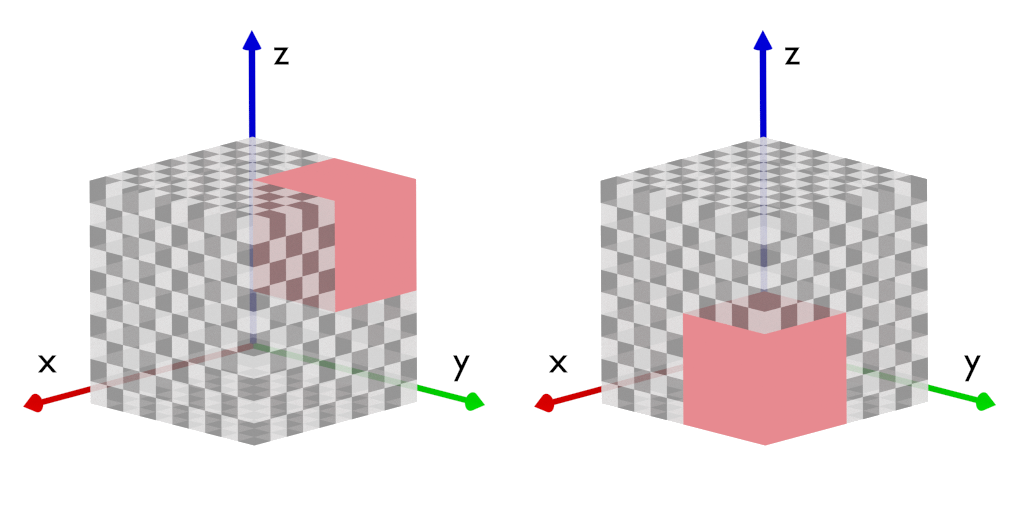
\includegraphics[width=.8\textwidth]{child_node_000_101.png}\\ % PNG-File
  \caption{Parent node (checkered) highlighted child nodes. Left: 000, right: 101}\label{fig:child_node_000_101.png}
\end{figure}

	\texttt{getNodeByIdentifierArray()} returns a reference to an \texttt{ocTree} object whose identifier matches the series of boolean values passed during the call. It mainly served testing and debugging purposes during development of the application, making sure the spatial indexing structure would be computed correctly for any given set of input 3D data. It is a utility function that provides fast, direct acces to any one desired node within an \texttt{ocTree} structure.

	\subsubsection{\texttt{buildTreeRecursively()}}
A call to this function will cause an entire set of given vertices to be indexed and assigned to a leaf node in the tree. Its only parameter required is an indexed list of vertices. A \texttt{std::vector<std::pair<size\_t, glm::vec3>>}, with the \texttt{size\_t} parts of the \texttt{pairs} providing ordered indexes and the \texttt{vec3} parts representing the vertices with three coordinates each, was used in this work.

	Most of what this function does, happens in a \texttt{for}-loop which iterates thorugh the entirety of the set of passed vertices. Its basic procedure is depicted in the following simplified C++ code snippet.

\begin{minipage}{\linewidth}
\begin{lstlisting}[language=C++,numberstyle=\zebra{black!5}{white}{},numbers=left,xleftmargin=2em,tabsize=3]
for(int t = 0; t != vertices.size(); ++t) {
	it = &vertices[t];
	if (it->second.x >= m_minX && it->second.x < m_maxX) {
		if (it->second.y >= m_minY && it->second.y < m_maxY) {
			if (it->second.z >= m_minZ && it->second.z < m_maxZ) {
				m_verticesInBounds.push_back(*it);
			}
		}
	}
}

if (m_verticesInBounds.size() > m_maxVerticesPerNode) {
		if (m_level < m_maxSplitDepth) {
			split();
		} else {
			std::cout << "EXCEPTION[...]" << std::endl;
			return false;
	}
}
\end{lstlisting}
\end{minipage}

Lines 1 - 10 check whether the current vertex lies within the bounds of the calling node. Note that each node calling this function will consider every vertex its parent node held in their member variable \texttt{m\_verticesInBounds}. In turn, if the calling node is to call \texttt{split()} later on, creating eight new subtree nodes, those nodes will consider each of the vertices that, via this loop have been determined to be located within their parent node. This stems from the trivial observation that a subtree can only contain vertices that are also contain by their parent node. So the root node of an \texttt{ocTree} will always check every single vertex of the loadedc 3D object but the higher their level, the subtree nodes will have to check fewer and fewer vertices.

Line 12 shows the crucial check wheter the number of vertices within the bounds of the calling node exceeds the maximum allowed number of vertices per node. If this is the case and the maximum allowed level (\texttt{m\_maxSplitDepth}) of subtrees is not reached yet (line 13), a call of \texttt{split()} by this node follows.

Figure \ref{fig:ocTree_levels.png} depicts a simple \texttt{ocTree} structure that could result from indexing a small set of 3D data. This particular tree has a root node at level zero, represented as a basic cube, in the upper left part of the figure. As the number of vertices within the bounds of the root exceeds the maximum numbers of vertices a node may hold in this particular tree, the root will call \texttt{split()} so that eight new subtrees are created and the root switches its boolean flag \texttt{isLeaf} to \texttt{false}, indicating that it is no longer a leaf node but the root of an actual subtree within the entire \texttt{ocTree}. Given that the maximum level of subtrees visible in the figure is 2, we assume that this is also the maximum allowed level for subtrees. This would mean that the identifier \texttt{vectors} of every node within this tree will have a length of $3*2$. The level 1 subtrees 000100 and 000111, as shown in the figure, also have more vertices within their bounds than what is the maximum number of vertices per node so they, too, split and created a total of 16 new child nodes, each at level 2.

\begin{figure}[htb]
  \centering
  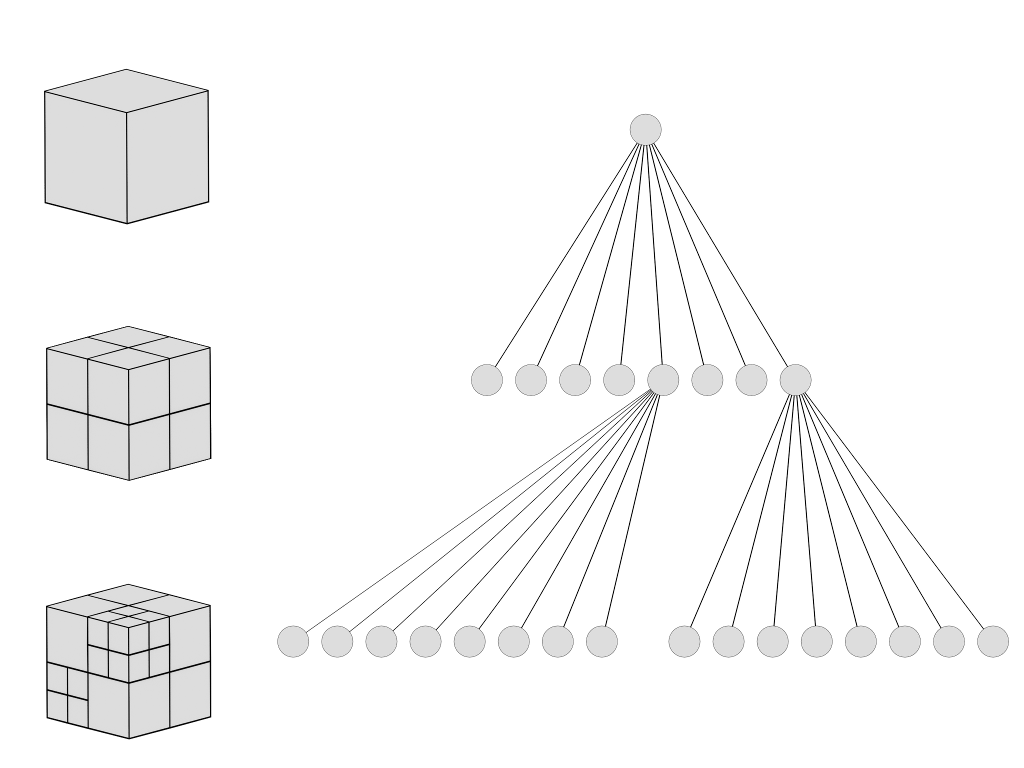
\includegraphics[width=0.95\textwidth]{ocTree_levels.png}
  \caption{depiction of a simple \texttt{ocTree}. Left: 3D view, step-wise representation of the splitting process (downwards from the top). right: final 2D representation of the tree's structure}\label{fig:ocTree_levels.png}
\end{figure}


\pagebreak % @TODO Das im Auge behalten!
\subsection{User Selection}
\label{sec:user_selection}

This section covers the elementary functions that handle the selection of vertices through user input. The two crucial functions explained in the subsequent subsections implement means to add vertices to an initially empty set of vertices and remove them later if desired. Selected vertices will be visually highlighted in the application and, at any time, the current set of selected vertices can be saved to an external text file.

	\subsubsection{\texttt{addVerticesToSelectionByCoordinates()}}

	\subsubsection{\texttt{removeVerticesFromSelectionByCoordinates()}}


\subsection{Tracking Selection}
\label{sec:tracking_selection}

\subsection{Testing Setup}
\label{sec:testing_setup}
This section will describe the steps I took to ensure that the selection application meets all its requirements and ensures its key features described above are implemented correclty.

% Testfile, Blender, etc
